\section{Performance Evaluation}\label{sec:pros_perf_eval}

\begin{marginfigure}[-1in]
\centerline{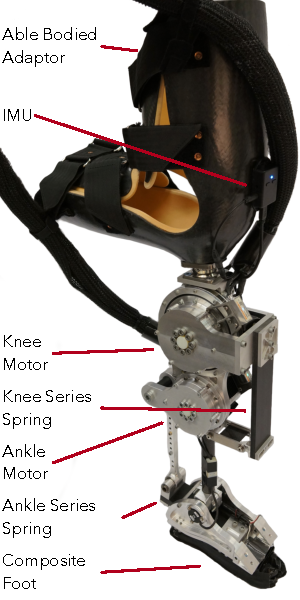
\includegraphics[width=\columnwidth]{pros_with_labels}}
\caption[Prosthesis configuration used for experiments]{Prosthesis configuration
used for experiments. An IMU attached on the thigh measures the thigh angle.
Note: the optional unidirectional ankle springs were not installed for
experiments presented in this thesis as the ankle motor alone produces
sufficient torque for the results presented
herein.}\label{fig:prosthesis_actual}
\end{marginfigure}

\Cref{fig:prosthesis_actual} shows the instantiation of the prosthesis design
used for the results presented in this thesis. As large ankle torques were not
required for the experiments conducted in this thesis, the optional
unidirectional ankle springs were not installed. Of crucial importance for the
work presented in this thesis is that the prosthesis faithfully reproduce the
torques commanded by the high level control. This is important so that we can
ensure differences between different high-level control strategies are due to
the differences in those strategies, and not due to an inability of the
prosthesis to follow the desired behaviors.

We test the ability of the manufactured prosthesis to reproduce desired torques
through three experiments: First, we collect data to construct a Bode plot of
the torque tracking behavior to confirm that the bandwidth of the actuators
exceeds the desired values in \cref{tab:pros_requirements}.  Second, we test the
ability of the prosthesis to track zero torque as a function of input
disturbance frequency. And third, we investigate the ability of the prosthesis
to follow the desired torques during a typical bout of walking.

\subsection{Torque Tracking Bode Plot}
\begin{figure}[htb]
\centerline{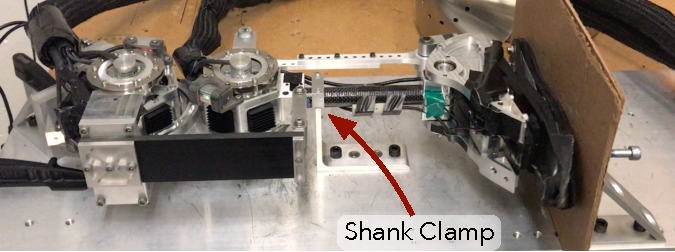
\includegraphics[width=\columnwidth]{bode_fixture}}
\caption[Fixture for testing bandwidth of actuators]{Fixture for testing
bandwidth of actuators. The knee was constrained by a clamp on the shank. The
ankle was constrained by a floor under the foot.}\label{fig:bode_fixture}
\end{figure}
To measure the torque tracking bandwidth of the prosthesis' knee and ankle
actuators, we construct bode plots of the transfer function between measured and
desired torque. For this purpose, we constrain the prosthesis in the fixture
shown in \cref{fig:bode_fixture}. In this fixture, the knee joint is
rotationally constrained by a clamp around the prosthesis' shank and the ankle
joint is constrained by a floor under the foot. To construct the bode plot, we
repeatedly command sinusoidal desired torques of varying frequencies $\omega$
and observe the resulting measured torques. We perform nonlinear least squares
regression to identify the amplitude and phase shift parameters of the function
$f(t) = A \sin(\omega t + \phi)$, where $A$ is the amplitude and $\phi$ is the
phase shift, such that the function fits the desired and measured torques.
Finally, we calculate the Gain, $G(\omega) = 20 \log_{10}
(\nicefrac{A_\tn{meas}}{A_\tn{des}})$ and the phase shift, $\phi(\omega) =
\phi_\tn{meas} - \phi_\tn{des}$, between the measured and desired signals at
each frequency. For both joints, we construct Bode plots at two amplitudes of
desired torque, a common amplitude of $\unit[20]{N \cdot m}$ and at the root
mean square (RMS) torques during stance for that joint ($\unit[11.5]{N \cdot m}$
for the knee, $\unit[55.6]{N \cdot m}$ for the ankle according to data from
\citet{bovi2011multiple} for \unit[80]{kg} person). For the knee joint we sweep
frequencies in the range \unit[1-35]{Hz} in \unit[1]{Hz} increments, and for the
ankle we sweep frequencies in the range \unit[1-20]{Hz}.

\begin{figure}[htb]
    \centering 
    \includegraphics[width=\textwidth]{bode_plot_fixed_labels}
    \caption[Experimentally obtained bode plots of knee and ankle actuator
    torque]{Experimentally obtained bode plots of knee and ankle actuator
    torque. Knee is phase limited at \unit[24]{Hz} while the ankle is gain
    limited at \unit[7]{Hz}.}\label{fig:pros_eval_bode_plots}
\end{figure}
\Cref{fig:pros_eval_bode_plots} shows the resulting knee and ankle bode plots at
the two tested amplitudes. We define the bandwidth of the actuator as the
frequency of the desired torque at which the gain falls below $\unit[-3]{dB}$ or
the phase lag falls below $\unit[-180]{deg}$, whichever comes first. We also
report the lower of the two bandwidth values obtained from the $\unit[20]{N
\cdot m}$ or RMS torques. For the knee joint, we see that the bandwidth is phase
limited at \unit[24]{Hz} by the $\unit[20]{N \cdot m}$ signal. The ankle
bandwidth is gain limited at \unit[7]{Hz} by the RMS stance torque signal. The
measured bandwidth of the knee and ankle actuators is higher than the desired
values based on able-bodied walking data (compare \cref{tab:pros_requirements}
desired knee bandwidth from \citep{sergi2012design}, desired ankle bandwidth
from \citet{au2008powered}).

\subsection{Zero Torque Tracking}
\begin{figure}[htb]
    \centering 
    \includegraphics[width=\textwidth]{zero_torque}
    \caption[Zero torque tracking of knee and ankle joints]{Zero torque tracking
    of knee and ankle joints. The prosthesis was fixed to a rigid mount and
    commanded to maintain zero net joint torque while the knee and ankle joints
    were manually oscillated (blue) by hand at increasingly fast rate (purple).
    The resulting measured torque is shown in the second row of axes in
    black.}\label{fig:pros_eval_zero_torque}
\end{figure}
Also important is the ability of the prosthesis to track the desired torque in
the presence of external disturbances. To test this ability, we removed the
shank clamp and floor from the fixture shown in \cref{fig:bode_fixture} and
commanded zero desired torque to the ankle and knee joints. We then manually
moved each joint in a sinusoidal motion while slowly increasing the frequency.
\Cref{fig:pros_eval_zero_torque} shows the angle of each joint during the
experiment and the approximate frequency of the motion, computed by inverting
the time between peaks of the joint angle. In the second row of plots, we show
the resulting measured torque. At \unit[3]{Hz} the peak knee torque is roughly
$\unit[6.5]{N \cdot m}$ and the peak ankle torque is roughly $\unit[20]{N \cdot
m}$. The knee peak knee torque is significantly less because knee actuator uses
a 50:1 gear reduction as opposed to a 100:1 reduction in the ankle, resulting in
less reflected inertia. The peak measured torque of both joints is less than
20\% of the peak torque during normal walking.

\subsection{Walking Torque Tracking}
\begin{figure}[htb]
    \centering 
    \includegraphics[width=\textwidth]{torque_tracking}
    \caption[Knee and ankle torque tracking during a typical step]{Knee and
    ankle torque tracking during a typical step. Torque tracking during stance
    is significantly better than during swing due to the significantly increased
    load inertia during stance (see \cref{tab:torque_tracking_tab}). During
    swing, trajectory tracking performance is
    prioritized.}\label{fig:torque_tracking_plot}
\end{figure}
Finally, we show the torque tracking performance of the prosthesis during normal
walking. \Cref{fig:torque_tracking_plot} shows the desired and measured torque
during a typical stride at a gait speed of \unitfrac[0.8]{m}{s} while
\cref{tab:torque_tracking_tab} shows the median RMS torque tracking error during
stance and swing over \unit[1]{min} of walking. For both joints we see that
torque tracking during stance is substantially better than during swing.  This
is the case for two reasons: First, during stance, the load inertia is
significantly increased, as it primarily is comprised of the mass of the user.
Consequently, the SEA dynamics are slower and easier to control. In contrast,
during swing, the load inertia is primarily the inertia of the prosthesis
itself. This primarily affects the ankle, as the inertia of the foot is
relatively small. Second, during swing the control's primary objective is to
follow a desired swing trajectory, (see \cref{sec:nm_control_prosthesis} for
more details). In this phase, the desired torque is generated by a PD feedback +
feedforward term to track the desired trajectory. Consequently, the desired
torques may not necessarily be feasible if the gains are high, as in the case of
the of desired ankle torque during swing.
\begin{margintable}[-1in]
    \centering
    \small
    \begin{tabular}{lcc}
        RMS Error (N-m) & Knee & Ankle \\
        \midrule
        Stance & 2.20 & 4.85  \\
        Swing  & 3.82 & 10.15 \\
    \end{tabular}
    \caption{Median root mean squared (RMS) torque tracking error during stance
    and swing}\label{tab:torque_tracking_tab}
\end{margintable}
